\documentclass{ximera}

%% You can put user macros here
%% However, you cannot make new environments

\listfiles

\graphicspath{{./}{firstExample/}{secondExample/}}

\usepackage{tikz}
\usepackage{tkz-euclide}
\usepackage{tikz-3dplot}
\usepackage{tikz-cd}
\usetikzlibrary{shapes.geometric}
\usetikzlibrary{arrows}
\usetikzlibrary{decorations.pathmorphing,patterns}
\usetkzobj{all}
\pgfplotsset{compat=1.13} % prevents compile error.

\renewcommand{\vec}[1]{\mathbf{#1}}
\newcommand{\RR}{\mathbb{R}}
\newcommand{\dfn}{\textit}
\newcommand{\dotp}{\cdot}
\newcommand{\id}{\text{id}}
\newcommand\norm[1]{\left\lVert#1\right\rVert}
 
\newtheorem{general}{Generalization}
\newtheorem{initprob}{Exploration Problem}

\tikzstyle geometryDiagrams=[ultra thick,color=blue!50!black]

\usepackage{mathtools}

\title{Direction Fields for First Order Equations}
\author{Adopted from Section 1.3 of W.F. Trench}

\begin{document}

\begin{abstract}
We define ordinary differential equations and what it means for a function to be a solution to such an equation.
\end{abstract}

\maketitle

\section*{Slope Fields for First Order Equations}

%this is Anna's addition to Trench

%Recall that, geometrically speaking, the value of the first derivative of a function at a point is the slope of the tangent line to the graph of the function at that point. So, given a differential equation of the form
%$$y'=f(x,y)$$
%we can interpret the value $f(a, b)$ as the slope of the tangent line to the graph of $y(x)$ at the point $(a, b)$.  For example, given the equation
%$$y'=x-y$$
%we know that the slope of the tangent line to the graph of a solution function at the point $(1,3)$ is $m=y'=1-3=-2$
%\begin{center}
%\begin{tikzpicture}[scale=1]
%\draw[thin,gray!40] (-4,-4) grid (4,4);
%  \draw[<->] (-4,0)--(4,0);
%  \draw[<->] (0,-4)--(0,4);
  
%  \draw[line width=2pt,red,-stealth](0,0)--(2,1) node[below right]{$\begin{bmatrix}2\\1\end{bmatrix}$};
%\draw[line width=2pt,red,-stealth, dashed](0,0)--(4,2) node[below right]{$2\begin{bmatrix}2\\1\end{bmatrix}$};
%  \draw[line width=2pt,blue,-stealth](0,0)--(2,-2) node[right]{$\begin{bmatrix}2\\-2\end{bmatrix}$};
% \draw[line width=2pt,blue,-stealth, dashed](0,0)--(-2,2) node[above left]{$(-1)\begin{bmatrix}2\\-2\end{bmatrix}$};
% \draw[line width=2pt,-stealth](0,0)--(2,4); 
%\end{tikzpicture}
%\end{center}

%So, the graph satisfying the initial condition $y(1)=3$ passes through the point $(1,3)$ in such a way that the tangent line to the graph has slope $m=-2$.

%another tikz

%Plotting multiple tangent lines helps us visualize what the solution curves might look like. Plotting tangent lines to solution curves at every point in the plane is impossible, but we can use technology to plot such tangent lines to some select points in the plane.  The resulting plot is called a \dfn{slope field}.  For example, the slope field for $y'=x-y$ looks like this:   

We cannot (yet!) solve the differential equation
\[
y' = x+y
\]
However, from the equation alone, we can deduce some facts about the
solution. Recall that, geometrically speaking, the value of the first derivative of a function at a point is the slope of the tangent line to the graph of the function at that point. So, given a differential equation of the form
\begin{equation}\label{eq:1.3.1}
y'=f(x,y)
\end{equation}
we can interpret the value $f(a, b)$ as the slope of the tangent line to the graph of $y(x)$ at the point $(a, b)$.
Thus, the differential equation
\[
y' = x+y
\]
tells us the \textbf{slope} of any solution passing through a given
point.
 
\begin{question}\label{quest:slopeAt1minus2}
  Consider the solution $y$ to the differential equation $y'=x+y$
  which passes through the point $(1,-2)$. What is the slope of the tangent line to
  solution $y$ at $x=1?$
    \begin{hint}
    By definition, a solution to this differential equation which
    passes through $(1,-2)$ must have $y(1)=-2$, and
    \begin{align*}
      y'(1) &= 1+y(-1)\\
      &= 1-2=-1.
    \end{align*}
    Hence the slope is $-1$ at $x=1$.
    \end{hint}
    \begin{prompt}
      The slope of $y$ at $x=1$ is $\answer{-1}$.
    \end{prompt}
\end{question} 
 
%\begin{exploration}\label{init:incDecSlopeField}
%  Consider the solution $y$ to the differential equation $y'=x+y$
%  which passes through the point $(1,2)$.  Is $y$ increasing or
%  decreasing at $x=1$?
%  \begin{prompt}
%  \begin{multipleChoice}
%    \choice[correct]{increasing}
%    \choice{decreasing}
%  \end{multipleChoice}
%  \end{prompt}
%  \begin{hint}
%    By definition, a solution to this differential equation which
%    passes through $(1,2)$ must have $y(1)=2$, and
%    \begin{align*}
 %     y'(1) &= 1+y(1)\\
 %     &=1+2\\
 %     &=3.
 %   \end{align*}
 %   This is positive, so the function is increasing at $x=1$.
 % \end{hint}
%\end{exploration}


 
Given a differential equation, say $y'=x+y$, we can pick points in the
plane and compute what the slope of a solution at those points will
be. Repeating this process, we can generate a \textit{slope field}.
The slope field for the differential equation $y' = x+y$ looks like
this:
\begin{image}
\begin{tikzpicture}
\def\length{sqrt(1+(x+y)^2)}
  \begin{axis}[
      xmin=-3, xmax=3,ymin=-3,ymax=3,domain=-3:3,view={0}{90},
      axis lines =center, xlabel=$x$, ylabel=$y$,
      every axis y label/.style={at=(current axis.above origin),anchor=south},
      every axis x label/.style={at=(current axis.right of origin),anchor=west},
      axis on top,
    ]
    \addplot3 [penColor, quiver={u={1/\length}, v={(x+y)/(\length)},scale arrows=.2},samples=20] {0};
]  \end{axis}
\end{tikzpicture}
\end{image}
 
Let's be explicit:
\begin{definition}
  A \dfn{slope field}, also called a \dfn{direction field}, is a
  graphical aid for understanding a differential equation, formed by:
  \begin{itemize}
    \item Choosing a grid of points.
    \item At each point, computing the slope given by the
          differential equation, using the $x$ and $y$-values of the
          point.
    \item At each point, drawing a short line segment with that
          slope.
\end{itemize}
\end{definition}
 
Here is the slope field for the differential equation $y'=x+y$, with a
few solutions of the differential equation also graphed.
 
\begin{image}
{\def\length{sqrt(1+(x+y)^2)}
\begin{tikzpicture}
  \begin{axis}[
      xmin=-3, xmax=3,ymin=-3,ymax=3,domain=-3:3,view={0}{90},
      axis lines =center, xlabel=$x$, ylabel=$y$,
      every axis y label/.style={at=(current axis.above origin),anchor=south},
      every axis x label/.style={at=(current axis.right of origin),anchor=west},
      axis on top,
    ]
    \addplot3 [penColor, quiver={u={1/\length}, v={(x+y)/(\length)},scale arrows=.2},samples=20] {0};
    \addplot[penColor,very thick]{e^x-x-1};
    \addplot[penColor,very thick]{.2*e^x-x-1};
    \addplot[penColor,very thick]{-e^x-x-1};
    \addplot[penColor,very thick]{-.2*e^x-x-1};
    \addplot[penColor,very thick]{-3*e^x-x-1};
    \addplot[penColor,very thick]{2*e^x-x-1};
    \addplot[penColor2,very thick]{-x-1};
]  \end{axis}
\end{tikzpicture}}
\end{image}

Each of the many solutions to the differential equation $y'=x+y$ is determined by initial conditions.  
The following interactive allows you to input the initial condition $(a, b)$ in the dialog box.  The output displays the slope field together with point $(a, b)$ and the solution that satisfies the initial condition.

\begin{sageCell}
@interact
def _(a=input_box(1, width=5),b=input_box(1, width=5)):
    x,y=var('x,y')
    v=plot_slope_field(x+y,(x,-5,5),(y,-5,5),headaxislength=3, headlength=3)
    c=(b+a+1)/(e^a)
    d=plot(c*e^x-x-1,(x,-5,1.5))
    p=point((a,b),rgbcolor=hue(1))
    show(v+d+p)
\end{sageCell}

\begin{question}\label{quest:slopefieldsguess}
Which of the five slope fields corresponds to the equation $y'=y^2$
\begin{multipleChoice}
\choice[correct]{
{\def\length{sqrt(1+(y^2+y)^2)}
\begin{tikzpicture}[framed,scale=.5,baseline=9ex]
  \begin{axis}[
      xmin=-3, xmax=3,ymin=-3,ymax=3,domain=-3:3,view={0}{90},
      axis lines =center, xlabel=$x$, ylabel=$y$,
      every axis y label/.style={at=(current axis.above origin),anchor=south},
      every axis x label/.style={at=(current axis.right of origin),anchor=west},
      axis on top,
    ]
    \addplot3 [penColor, quiver={u={1/\length}, v={(y^2)/(\length)},scale arrows=.2},samples=20] {0};
]  \end{axis}
\end{tikzpicture}}}
 
\choice{{\def\length{sqrt(1+(x-y)^2)}
\begin{tikzpicture}[framed,scale=.5,baseline=9ex]
  \begin{axis}[
      xmin=-3, xmax=3,ymin=-3,ymax=3,domain=-3:3,view={0}{90},
      axis lines =center, xlabel=$x$, ylabel=$y$,
      every axis y label/.style={at=(current axis.above origin),anchor=south},
      every axis x label/.style={at=(current axis.right of origin),anchor=west},
      axis on top,
    ]
    \addplot3 [penColor, quiver={u={1/\length}, v={(x-y)/(\length)},scale arrows=.2},samples=20] {0};
]  \end{axis}
\end{tikzpicture}}}
 
\choice{{\def\length{sqrt(1+(x)^2)}
\begin{tikzpicture}[framed,scale=.5,baseline=9ex]
  \begin{axis}[
      xmin=-3, xmax=3,ymin=-3,ymax=3,domain=-3:3,view={0}{90},
      axis lines =center, xlabel=$x$, ylabel=$y$,
      every axis y label/.style={at=(current axis.above origin),anchor=south},
      every axis x label/.style={at=(current axis.right of origin),anchor=west},
      axis on top,
    ]
    \addplot3 [penColor, quiver={u={1/\length}, v={(x^2)/(\length)},scale arrows=.2},samples=20] {0};
]  \end{axis}
\end{tikzpicture}}}
 
\choice{{\def\length{sqrt(1+(y)^2)}
\begin{tikzpicture}[framed,scale=.5,baseline=9ex]
  \begin{axis}[
      xmin=-3, xmax=3,ymin=-3,ymax=3,domain=-3:3,view={0}{90},
      axis lines =center, xlabel=$x$, ylabel=$y$,
      every axis y label/.style={at=(current axis.above origin),anchor=south},
      every axis x label/.style={at=(current axis.right of origin),anchor=west},
      axis on top,
    ]
    \addplot3 [penColor, quiver={u={1/\length}, v={(x)/(\length)},scale arrows=.2},samples=20] {0};
]  \end{axis}
\end{tikzpicture}}}
 
\choice{{\def\length{sqrt(1+(-x/y)^2)}
\begin{tikzpicture}[framed,scale=.5,baseline=9ex]
  \begin{axis}[
      xmin=-3, xmax=3,ymin=-3,ymax=3,domain=-3:3,view={0}{90},
      axis lines =center, xlabel=$x$, ylabel=$y$,
      every axis y label/.style={at=(current axis.above origin),anchor=south},
      every axis x label/.style={at=(current axis.right of origin),anchor=west},
      axis on top,
    ]
    \addplot3 [penColor, quiver={u={1/\length}, v={(-x/y)/(\length)},scale arrows=.2},samples=20] {0};
]  \end{axis}
\end{tikzpicture}}}
\end{multipleChoice}
\begin{hint}
  Consider slopes of tangent lines in key areas, such as the origin, each of the four quadrants.  Are the slopes getting steeper as $x$ or $y$ increase?
\end{hint}

\end{question}

%\begin{sageCell}
%x,y=var('x, y')
%v=plot_slope_field((x-y),(x,-1,1),(y,-1,1),headaxislength=3, headlength=3)
%show(v)
%\end{sageCell}

%Anna's text transitions into Trench.
Given a differential equation such as $y'=x+y$ it is easy to find an explicit solution to the equation.  (You may want to verify that functions of the form $y=ce^x-x-1$ are solutions.)  However, it's impossible to find explicit formulas for solutions of some
differential equations. Even if there are such  formulas, they may be
so complicated that they're useless. In this case we may resort to
graphical or numerical methods to get some idea of how the solutions
of the given equation behave. Slope fields offer us one such method.

% {\color{red}In a later module} we'll take up
%the question of existence of solutions of a first order equation
%\begin{equation} \label{eq:1.3.1}
%y'=f(x,y).
%\end{equation}
%In this section we'll simply assume that \eqref{eq:1.3.1} has
%solutions and discuss a graphical method for approximating them.
%In {\color{red}Chapter~3} we discuss numerical methods for obtaining
%approximate solutions of \eqref{eq:1.3.1}.

%Recall that a solution of \eqref{eq:1.3.1} is a function $y=y(x)$ such
%that
%$$
%y'(x)=f(x,y(x))
%$$
%for all values of $x$ in some interval, and an integral curve is
%either the graph of a solution or is
%made up of  segments that are graphs of solutions.
% Therefore, not being able to
%solve \eqref{eq:1.3.1} is equivalent to not knowing the equations of
%integral curves of \eqref{eq:1.3.1}. However, it's easy to calculate the
%slopes of these curves. To be specific, the slope of an integral curve
%of \eqref{eq:1.3.1} through a given point $(x_0,y_0)$ is given by the
%number $f(x_0,y_0)$. This is the basis of \dfn{the method of direction fields}.

%If $f$ is defined on a set $R$, we can construct a direction
%field for \eqref{eq:1.3.1}  in $R$ by drawing a
%short
%line segment through each point $(x,y)$ in $R$ with slope $f(x,y)$. Of
%course, as a practical matter, we can't actually draw line segments
%through {\color{blue}\it every\/} point in $R$;     rather, we must select
%a finite
%set of points in $R$. For example, suppose   $f$ is defined on the
%closed rectangular region
%$$
%R:\{a\le x\le b, c\le y\le d\}.
%$$
%Let
%$$
%a= x_0< x_1< \cdots< x_m=b
%$$
%be  equally spaced points in $[a,b]$ and
%$$
%c=y_0<y_1<\cdots<y_n=d
%$$
%be  equally spaced points in $[c,d]$.
% We say that the points
%$$
 %(x_i,y_j),\quad 0\le i\le m,\quad 0\le j\le n,
%$$
%form a {\color{blue}\it rectangular grid\/} (Figure~\ref{figure:1.3.1}). Through each
%point in the grid we draw a short line segment with slope
%$f(x_i,y_j)$. The result is an approximation to a direction field  for
%\eqref{eq:1.3.1} in $R$. If the grid points are sufficiently numerous and
%close together, we can draw approximate integral curves of \eqref{eq:1.3.1}
%by drawing curves through points in the grid tangent to the line
%segments associated with the points in the grid.

%Unfortunately, approximating a direction field and graphing integral
%curves in this way is too tedious to be done effectively by hand.
%However, there is software  for doing this.
As you'll  see, the combination of  direction fields and
 integral curves gives  useful insights into the behavior of
the solutions of the differential equation even if
we can't obtain exact solutions.

We'll  study numerical methods for solving a single first order
equation \eqref{eq:1.3.1} in {\color{red}Chapter~3}. These methods can be
used
to plot solution curves of \eqref{eq:1.3.1} in a rectangular region $R$ if $f$ is continuous on $R$. The figures in the three examples below show direction fields and solution
curves for several differential equations of the form \eqref{eq:1.3.1} with $f$
 continuous for all $(x,y)$.
 \begin{example}\label{ex:fig010302}
$$
 y'=\frac{x^2-y^2}{1+x^2+y^2}
 $$
 \begin{image}
  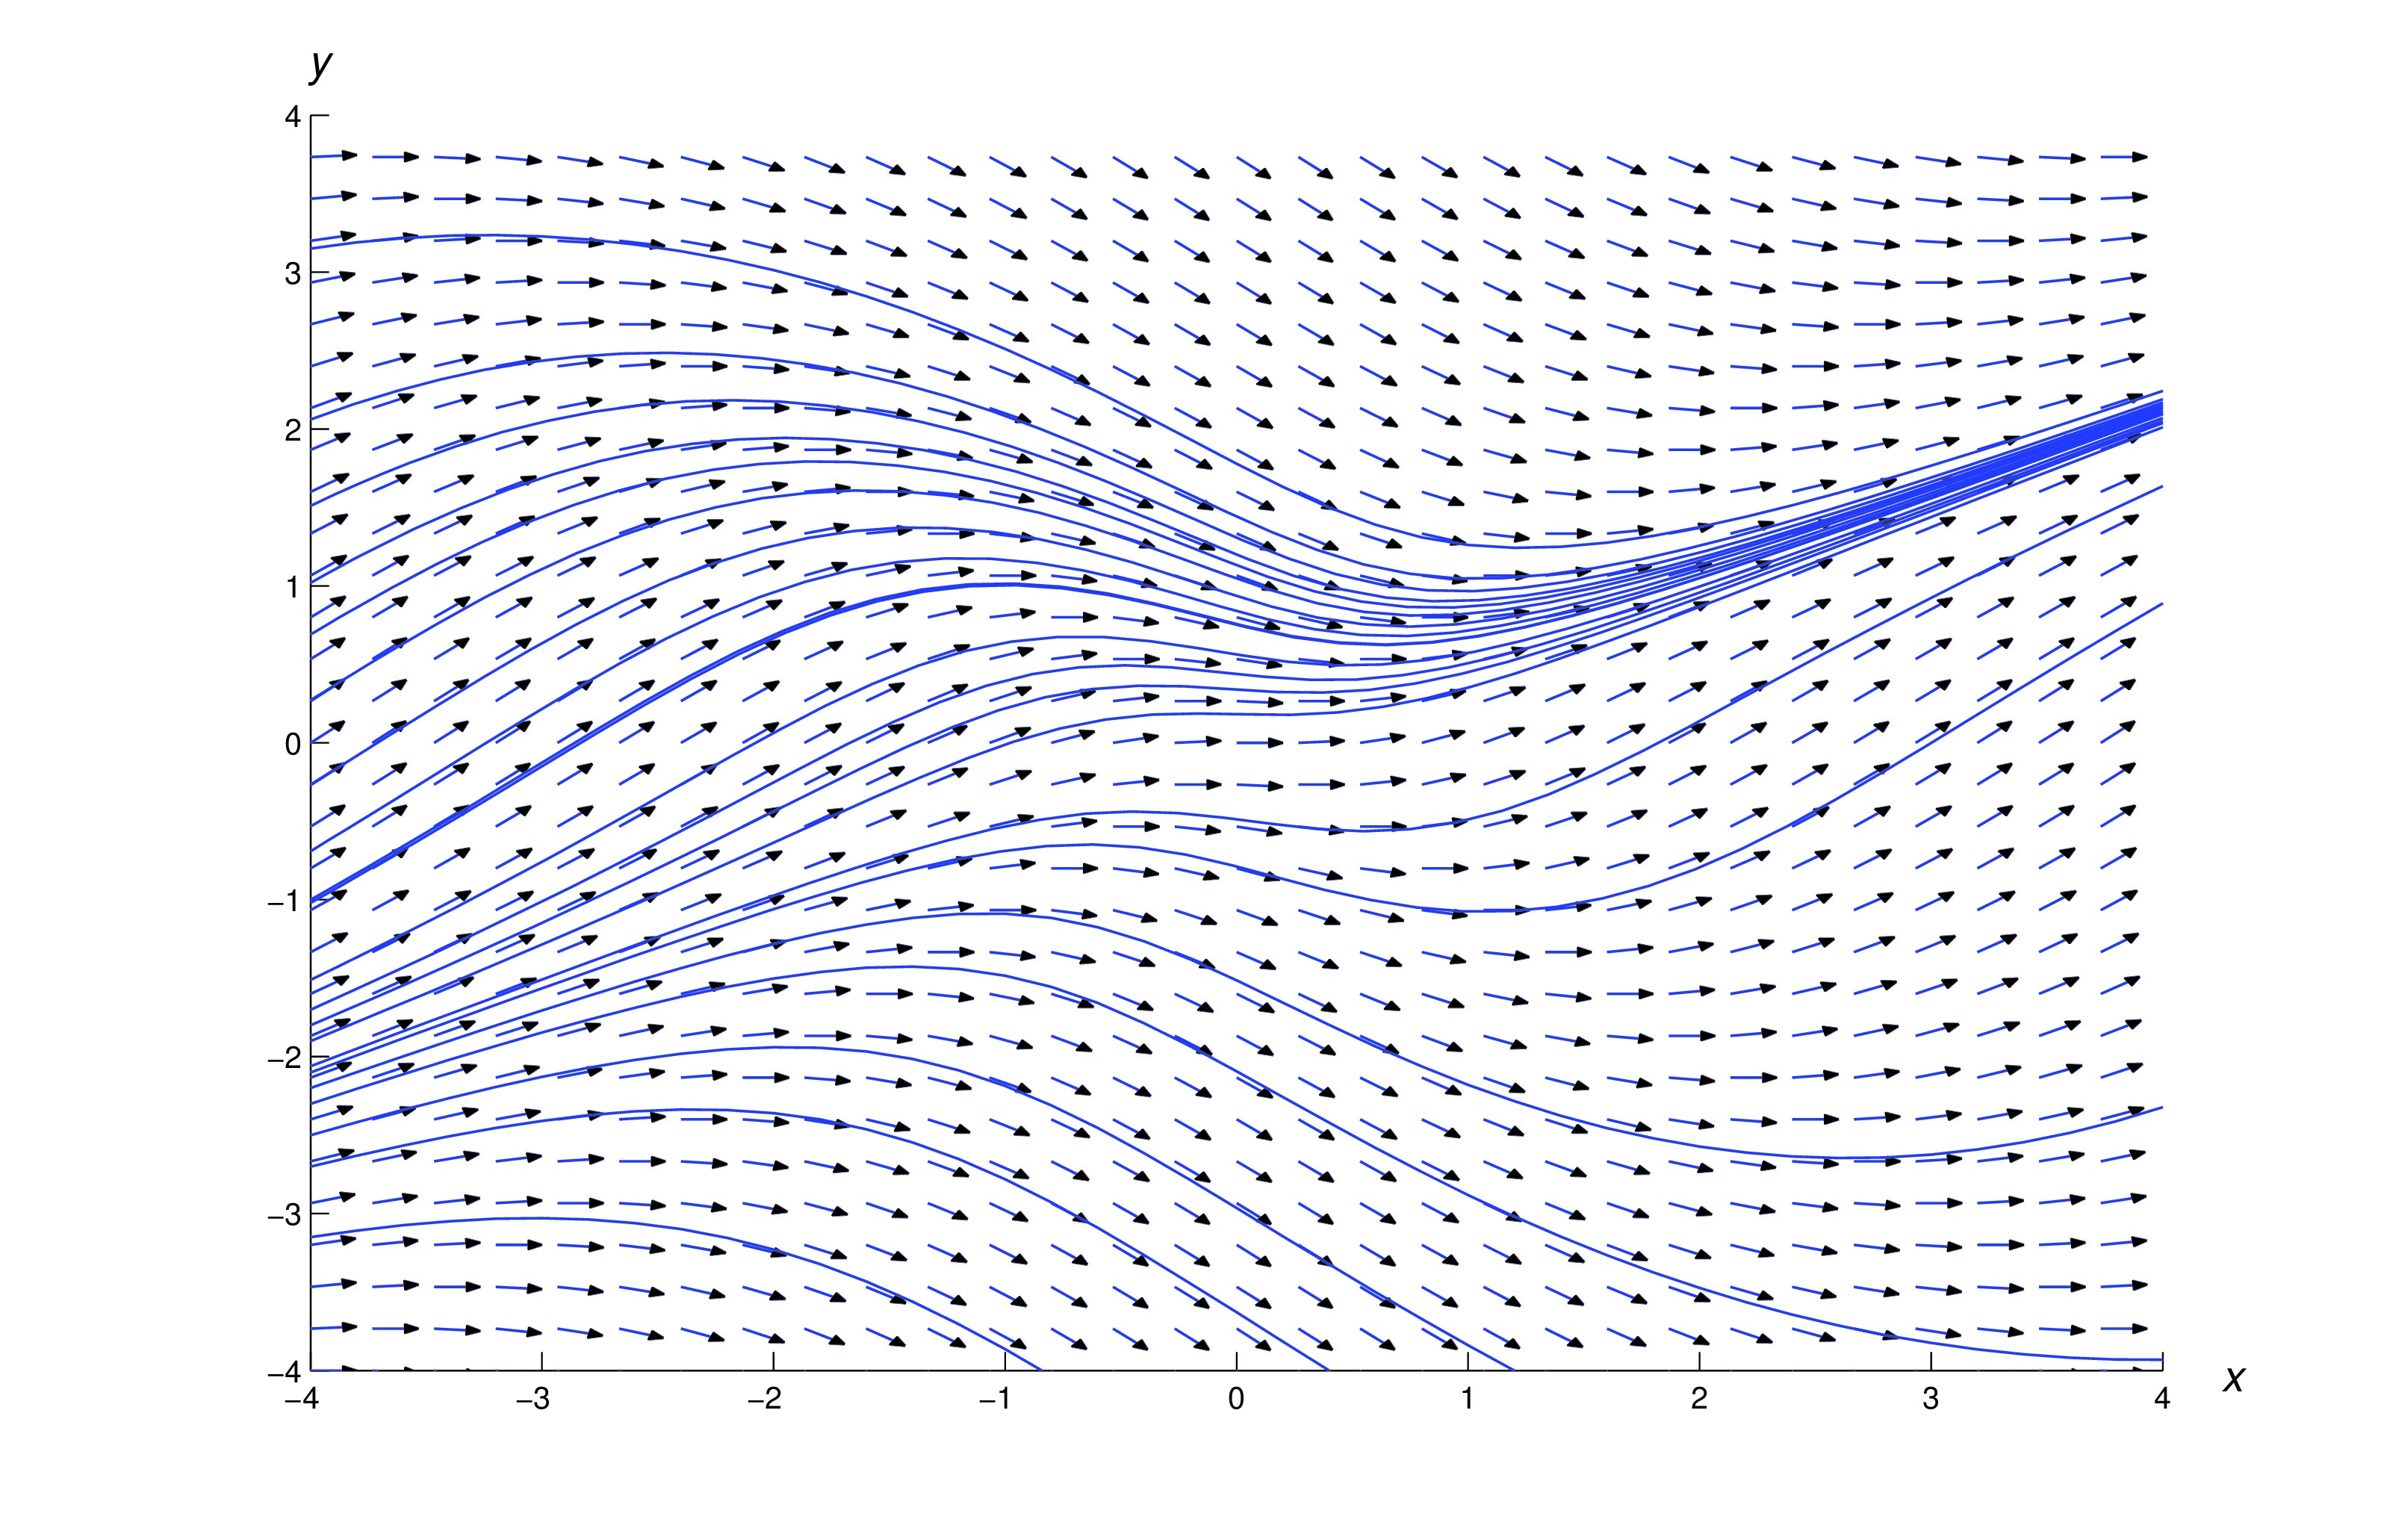
\includegraphics{fig010302.jpg}
\end{image}
\end{example}

\begin{example}\label{ex:fig010303}
$$
y'=1+xy^2
$$
\begin{image}
  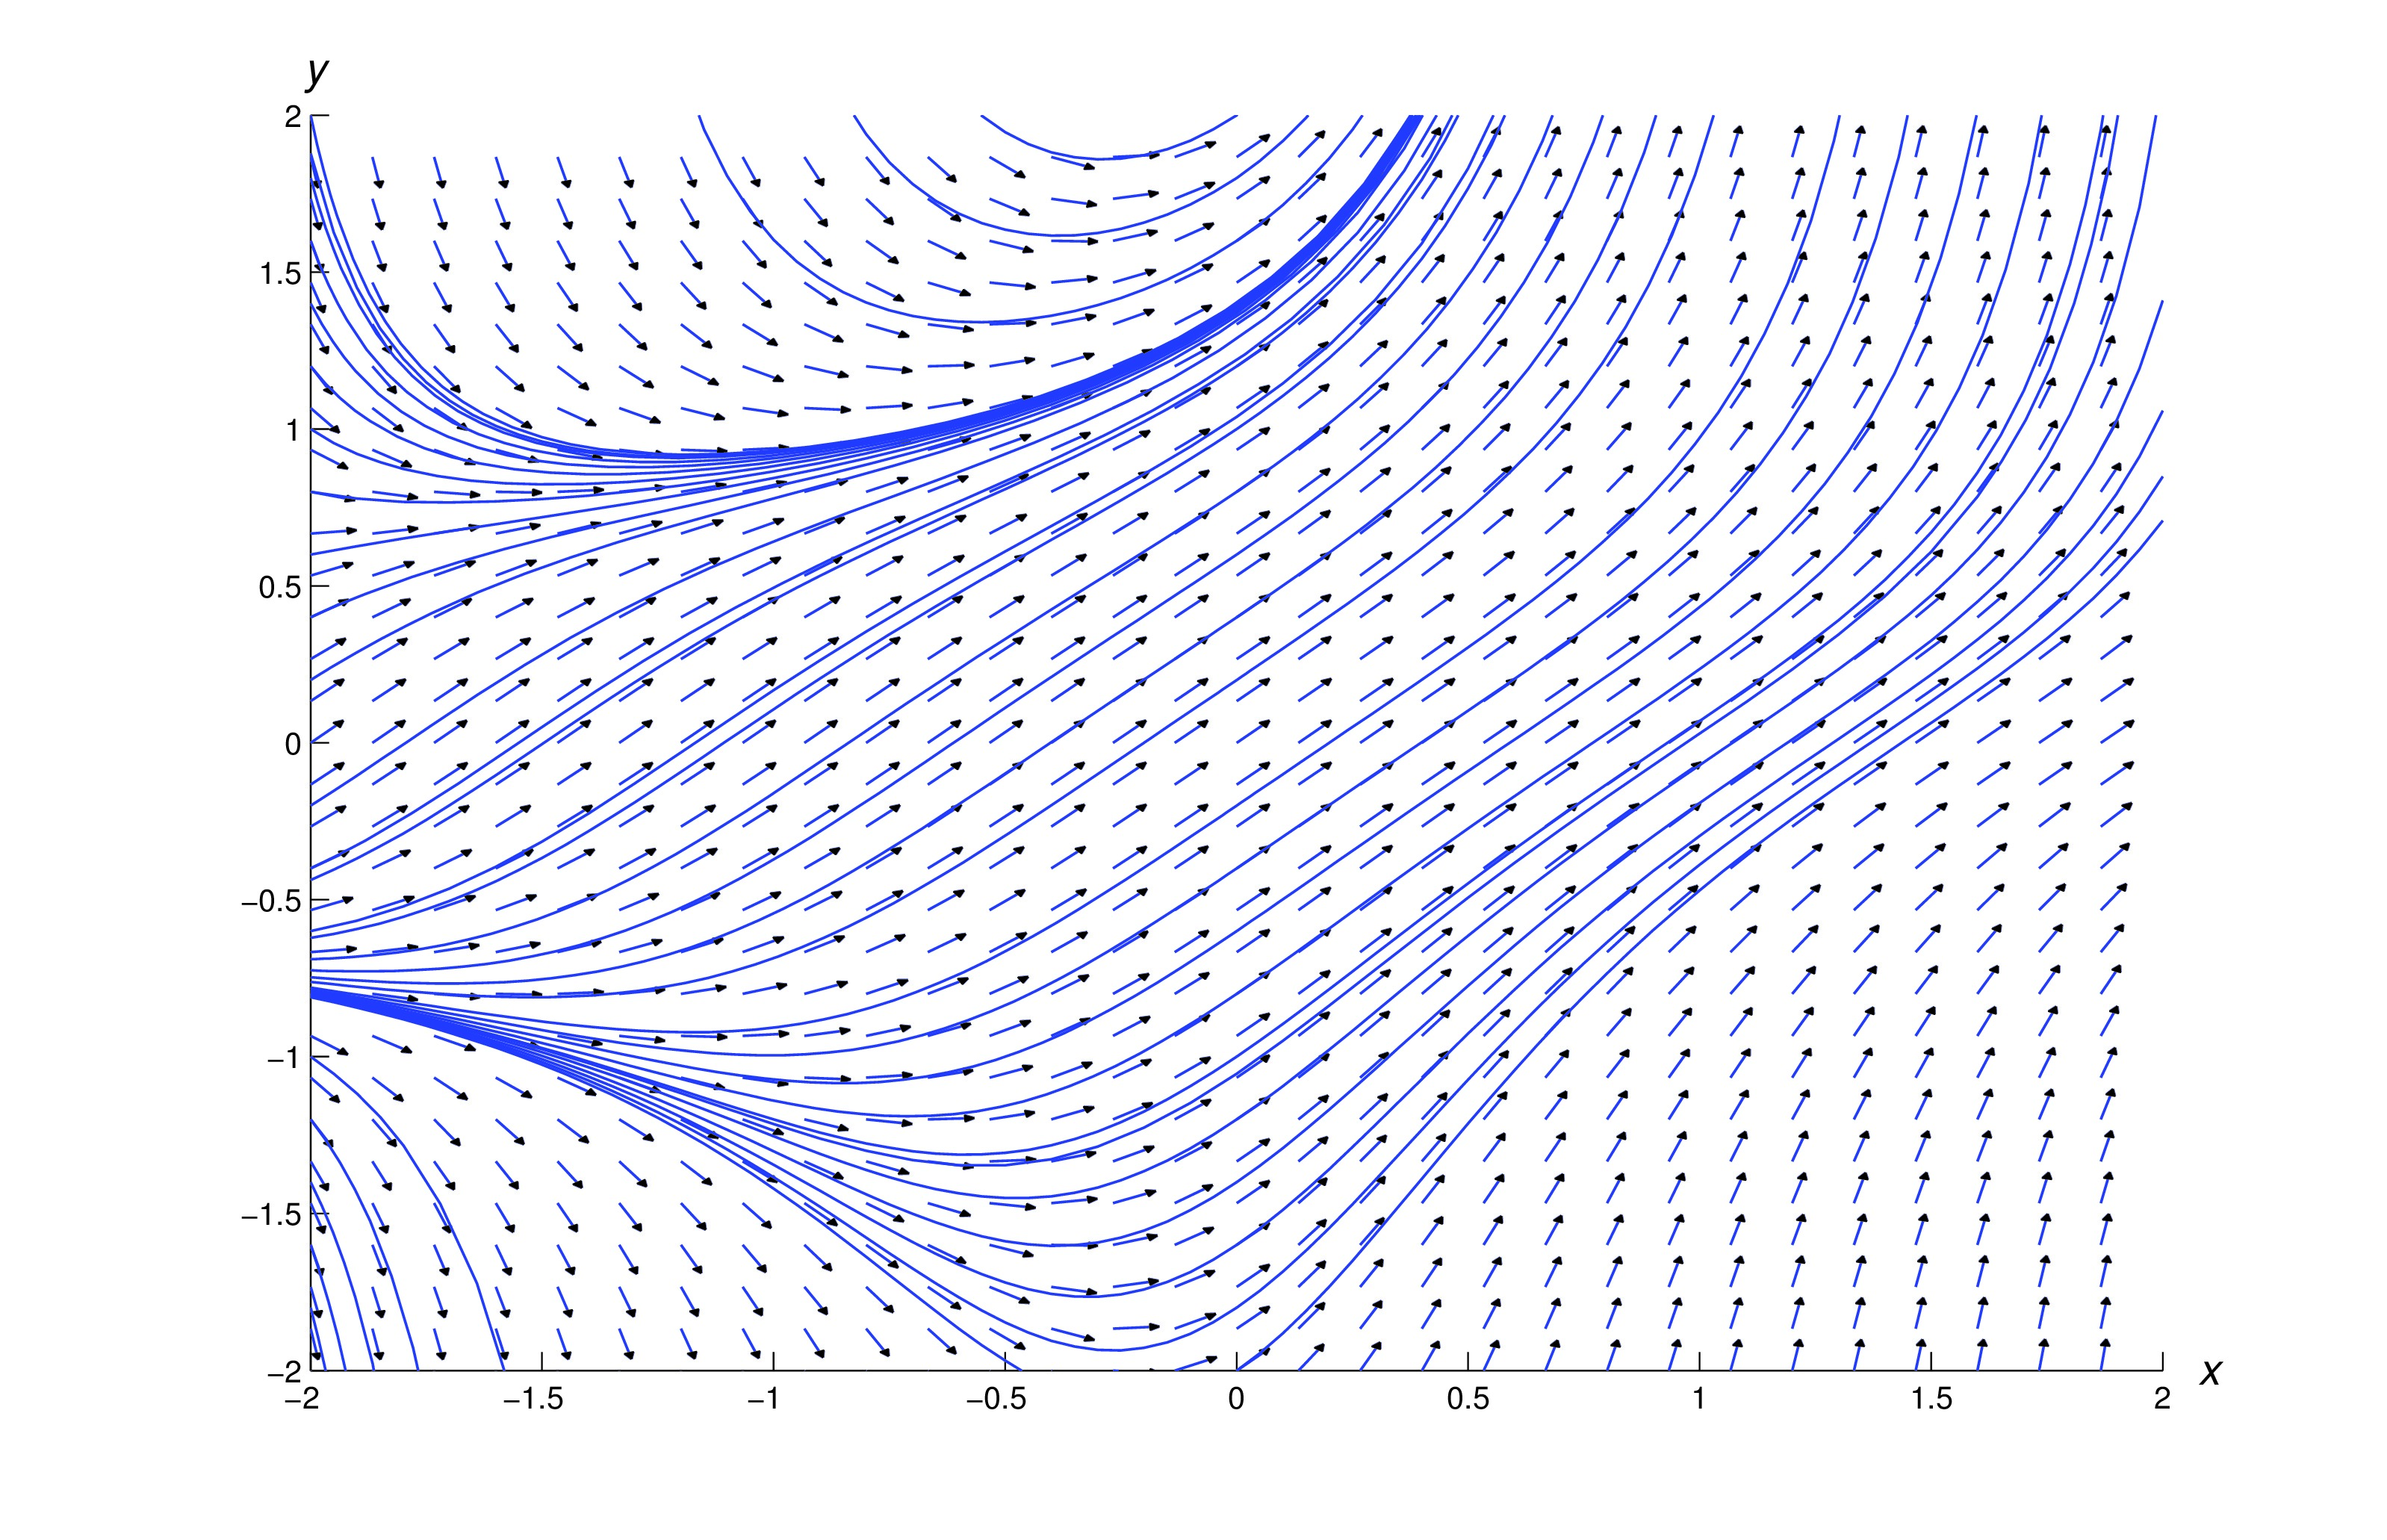
\includegraphics{fig010303.jpg}
\end{image}
\end{example}
\begin{example}\label{ex:fig010304}
$$
y'=\frac{x-y}{1+x^2}
$$
\begin{image}
   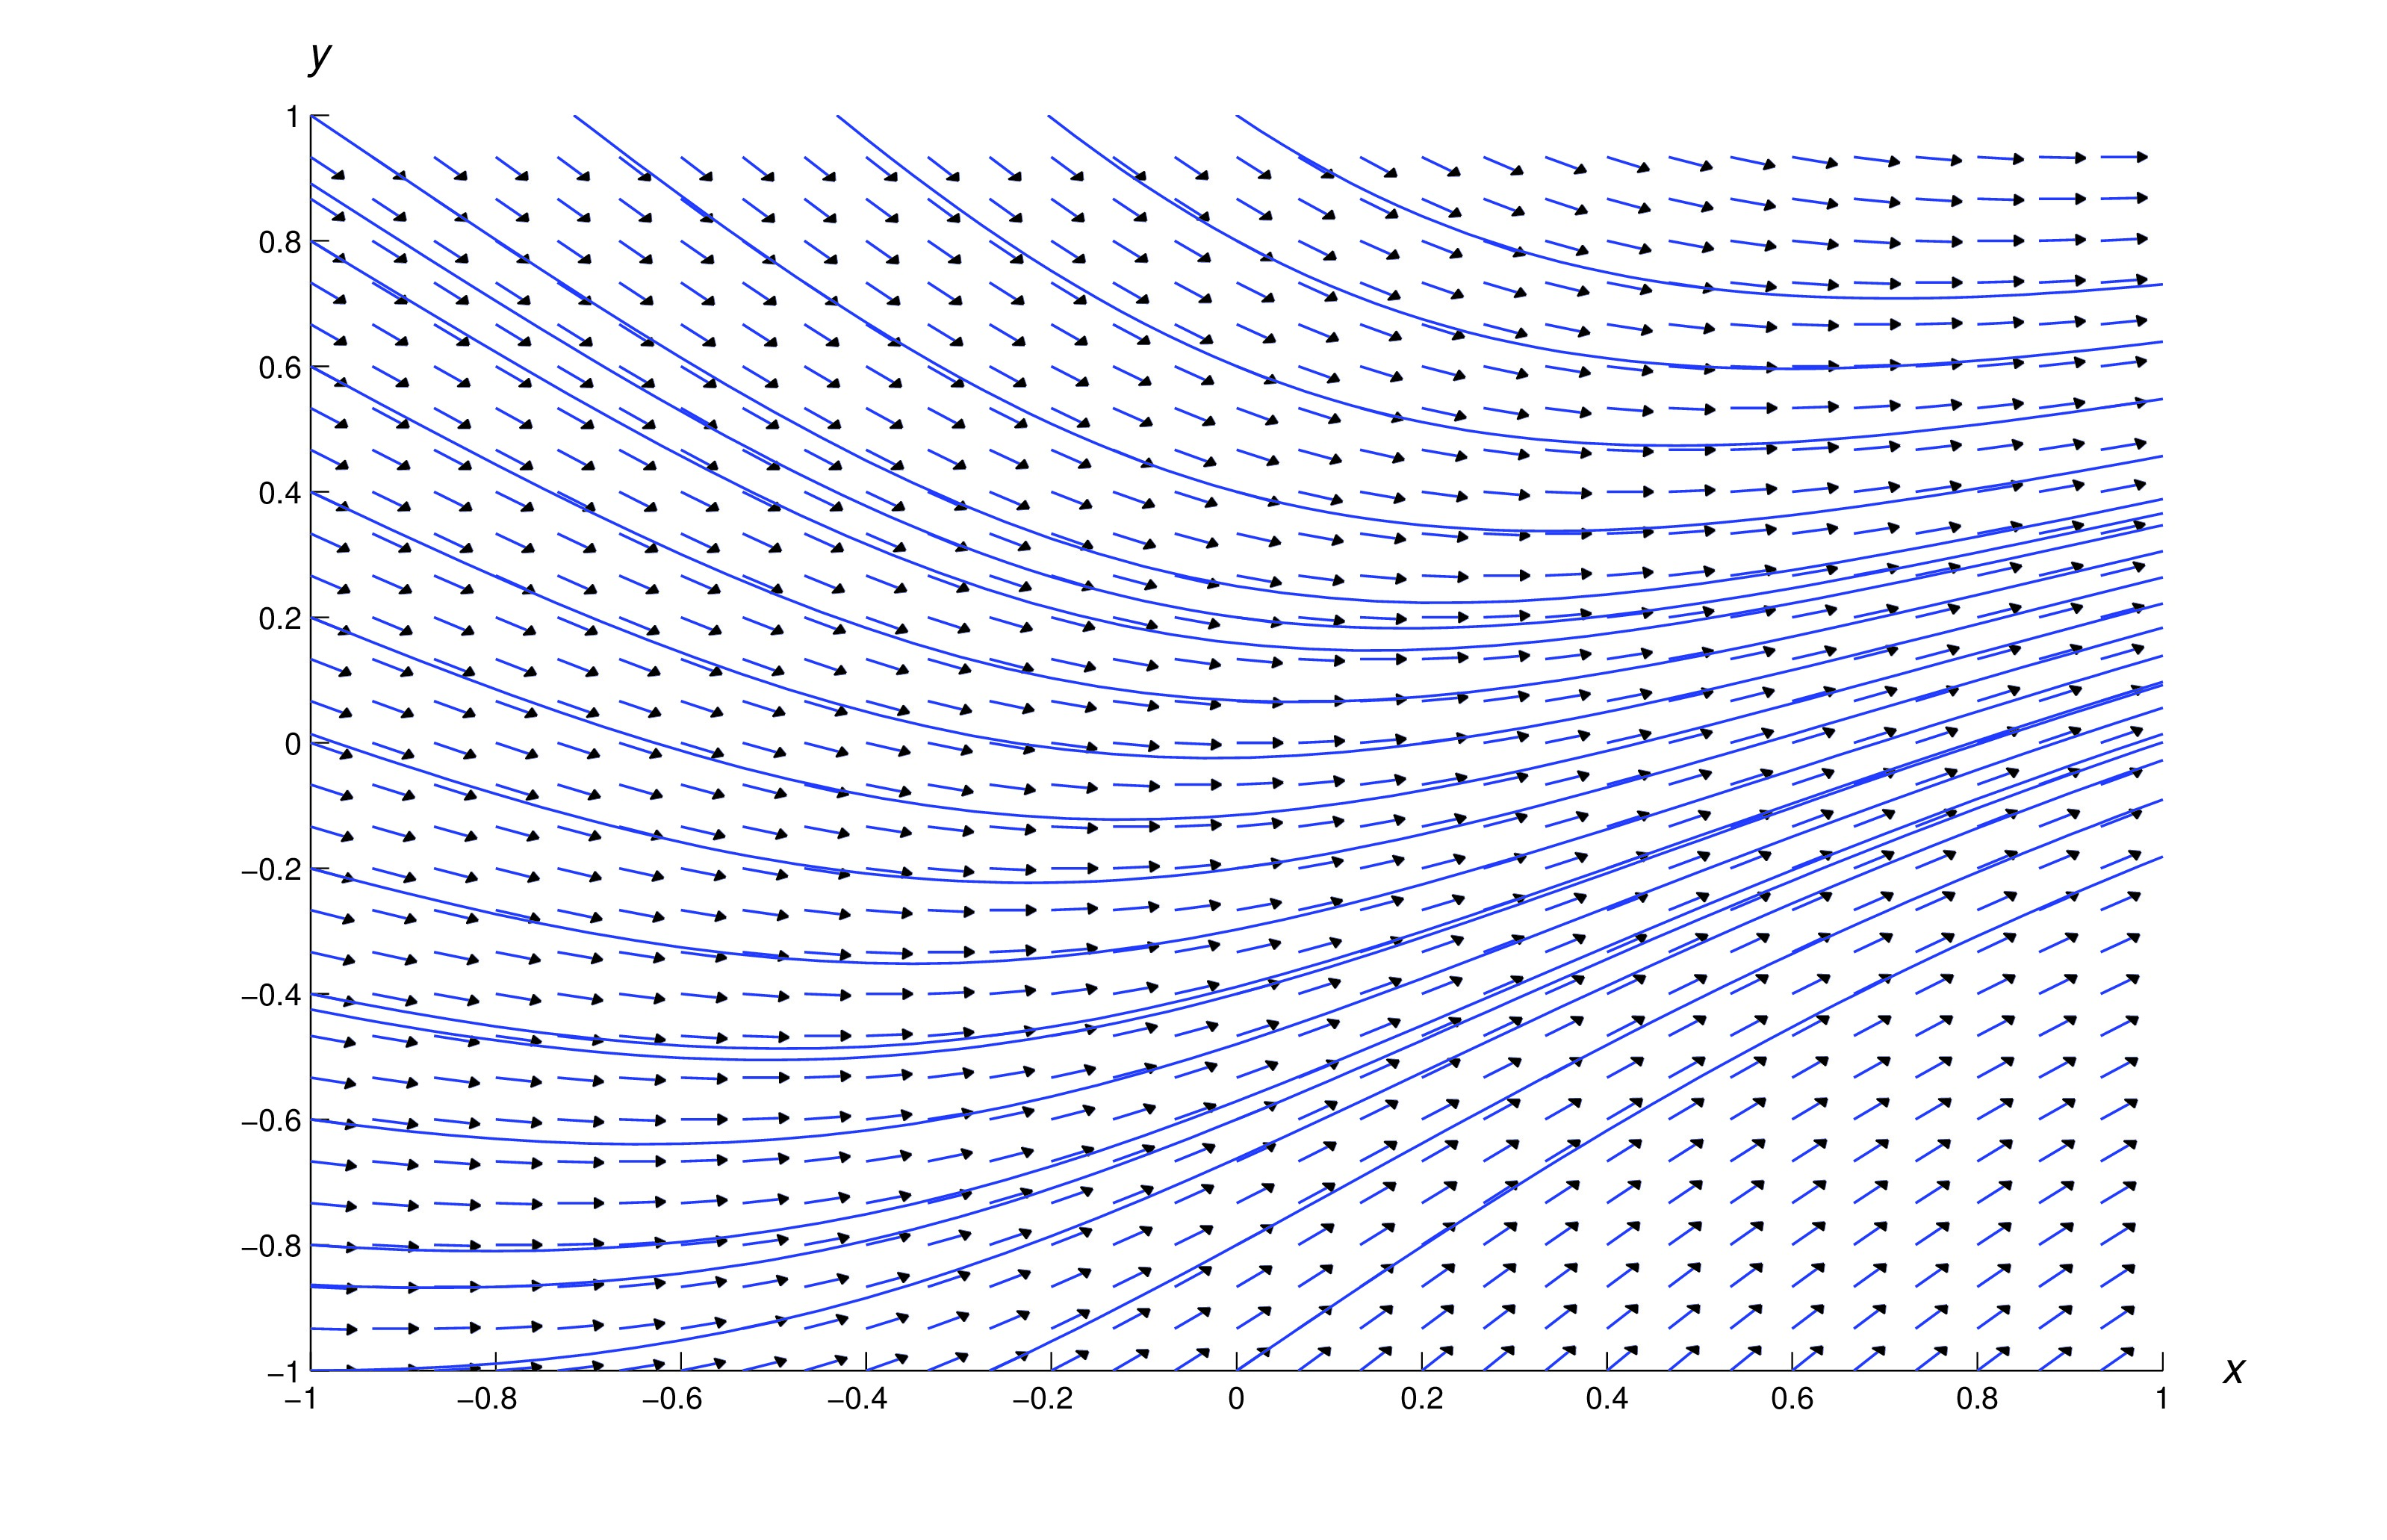
\includegraphics{fig010304.jpg}
\end{image}
\end{example}
The methods of {\color{red}Chapter~3} won't work for the equation
\begin{equation} \label{eq:1.3.2}
y'=-\frac{x}{y}
\end{equation}
if $R$ contains part of the $x$-axis, since $f(x,y)=-x/y$ is undefined
when $y=0$. Similarly, they won't work for the equation
\begin{equation} \label{eq:1.3.3}
y'=\frac{x^2}{1-x^2-y^2}
\end{equation}
if $R$ contains any part of the unit circle $x^2+y^2=1$, because the
right side of \eqref{eq:1.3.3} is undefined if $x^2+y^2=1$. However,
\eqref{eq:1.3.2} and \eqref{eq:1.3.3} can written as
\begin{equation} \label{eq:1.3.4}
y'=\frac{A(x,y)}{B(x,y)}
\end{equation}
where $A$ and $B$ are  continuous on any rectangle $R$. Because of
this,
some differential equation software is based on
numerically solving pairs of equations of the form
\begin{equation} \label{eq:1.3.5}
\frac{dx}{dt}=B(x,y),\quad \frac{dy}{dt}=A(x,y)
\end{equation}
where $x$ and $y$ are regarded as functions of a parameter $t$.
If $x=x(t)$ and $y=y(t)$  satisfy these equations, then
$$
y'=\frac{dy}{dx}=\frac{\frac{dy}{dt}}{\frac{dx}{dt}}=\frac{A(x,y)}{B(x,y)},
$$
so $y=y(x)$ satisfies \eqref{eq:1.3.4}.

Eqns.~\eqref{eq:1.3.2} and \eqref{eq:1.3.3} can be reformulated as in
\eqref{eq:1.3.4} with
$$
\frac{dx}{dt}=-y,\quad \frac{dy}{dt}=x
$$
and
$$
\frac{dx}{dt}=1-x^2-y^2,\quad \frac{dy}{dt}=x^2,
$$
respectively. 

The figure below shows a direction field and some integral curves
for $y'=-\frac{x}{y}$. As we saw in
Example~\ref{example:1.2.1}, the integral curves of \eqref{eq:1.3.2}
are circles centered at the origin.

\begin{image}
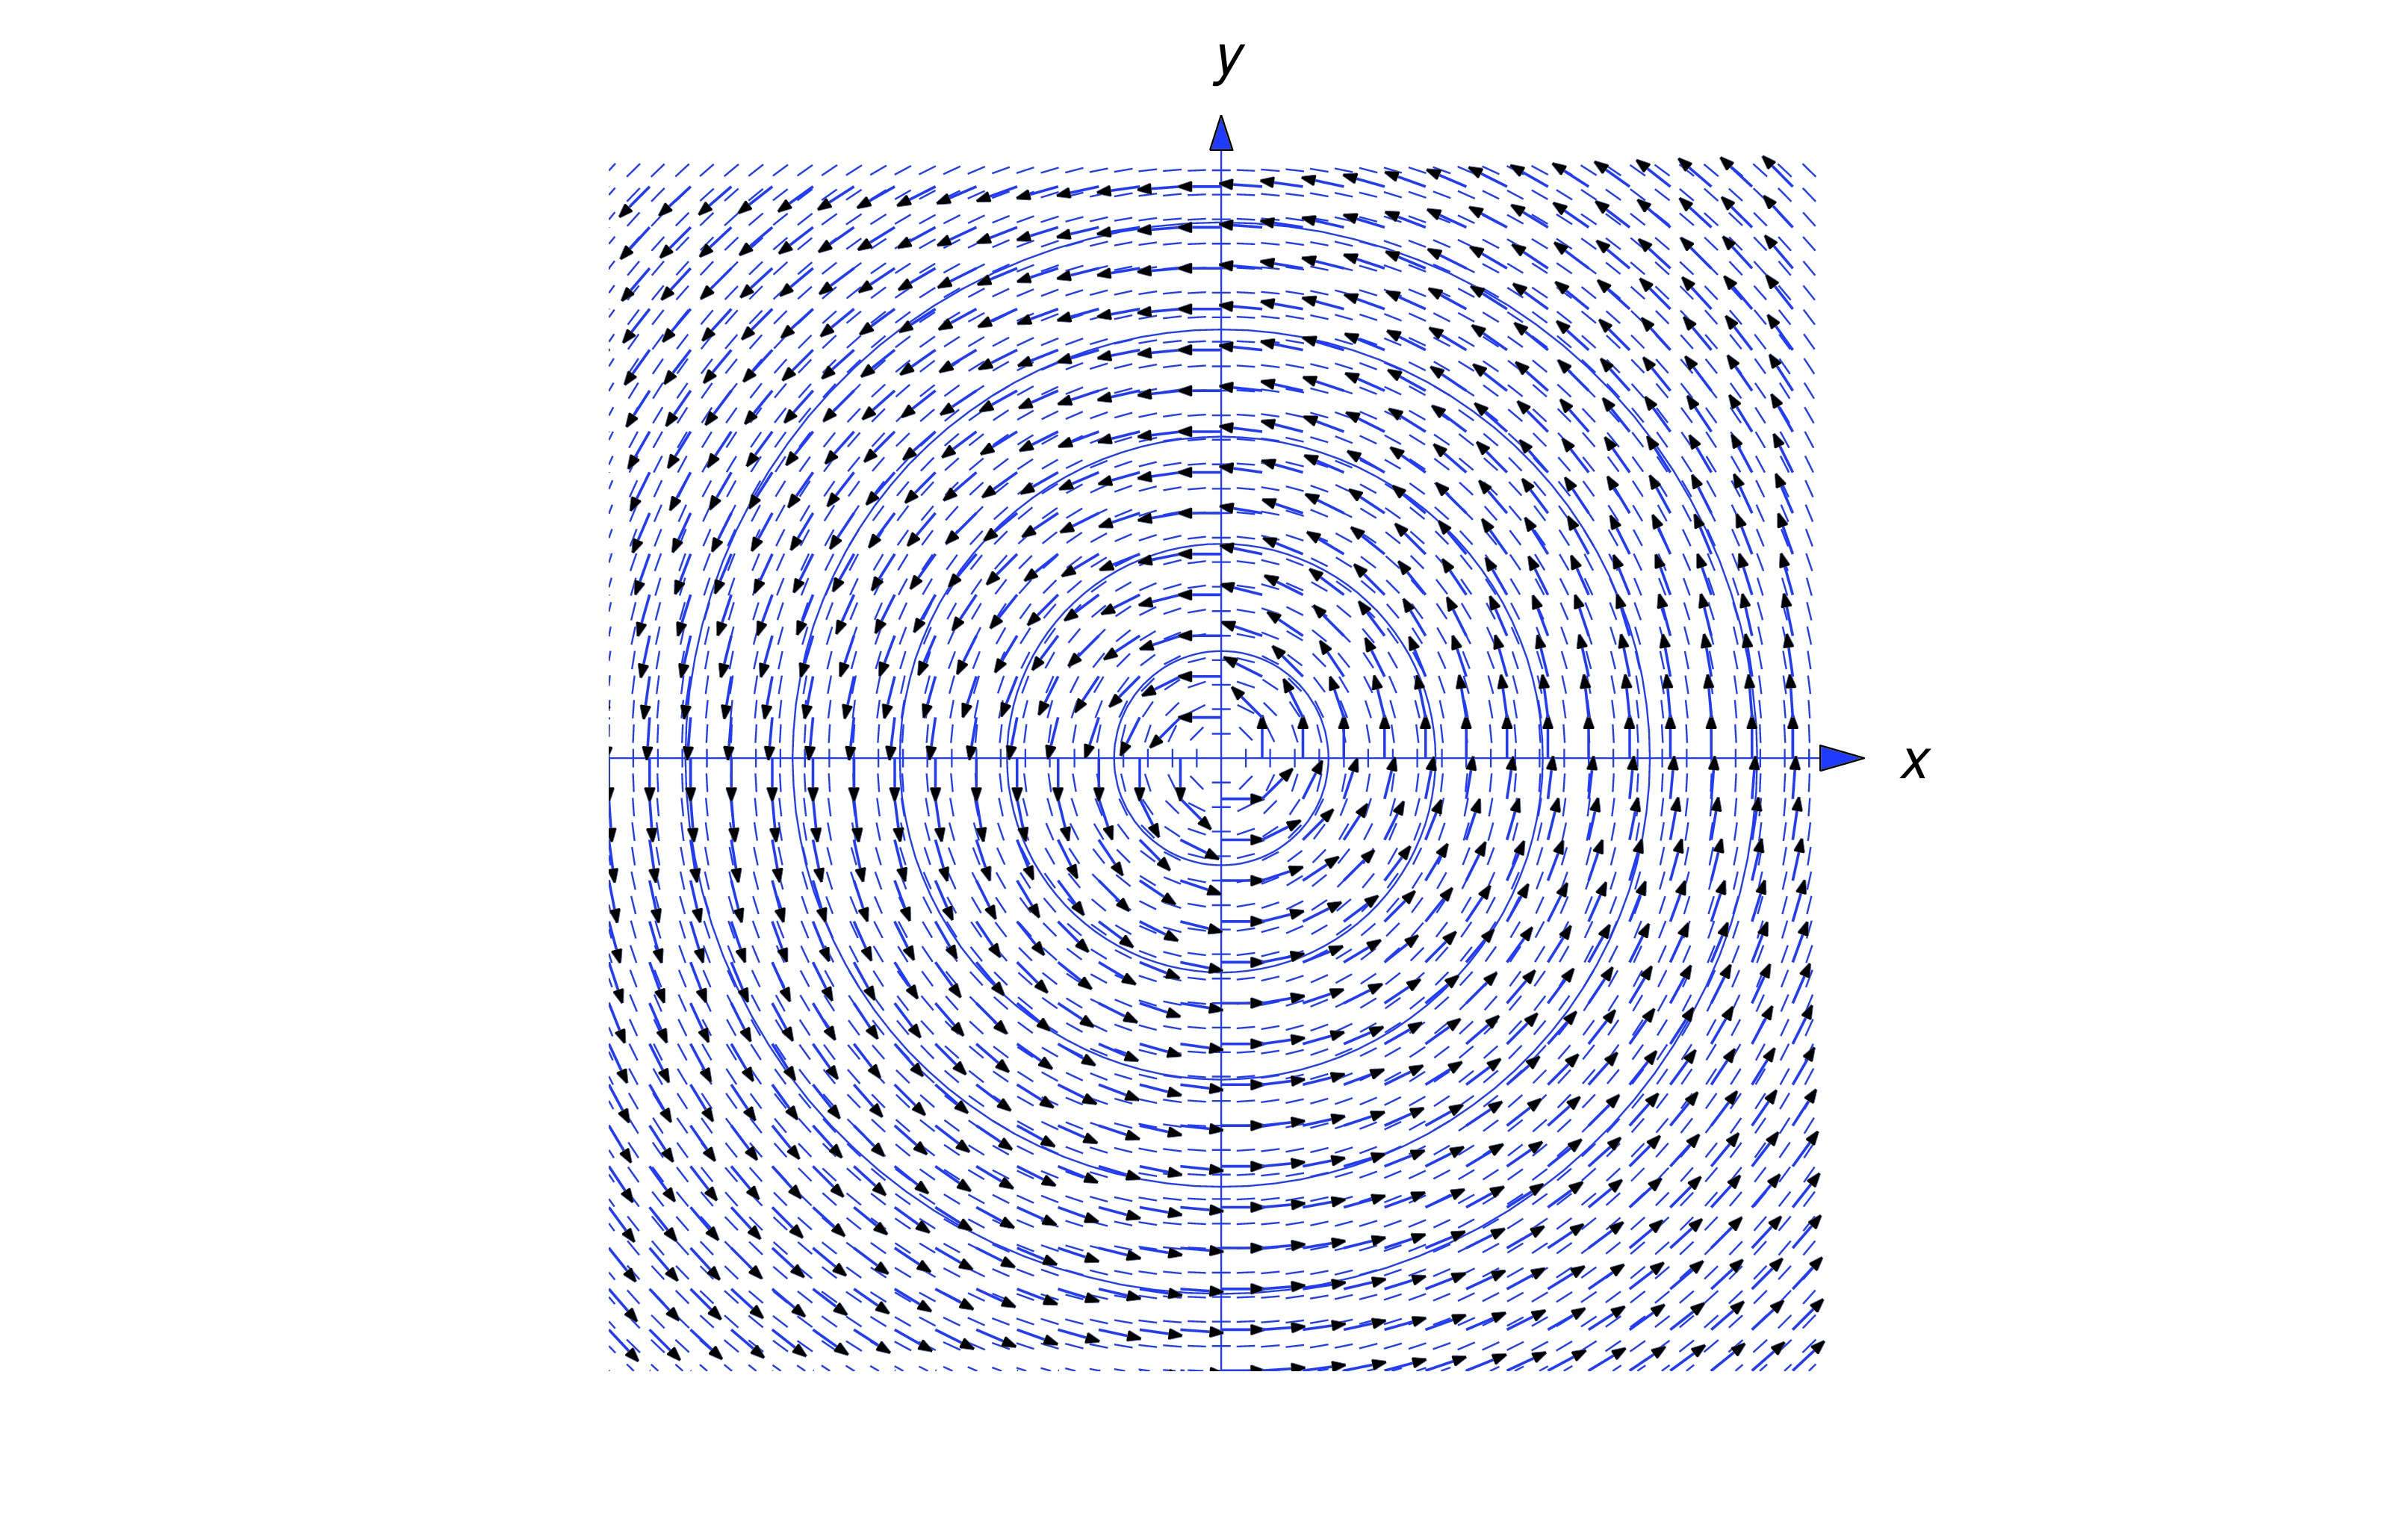
\includegraphics{fig010305.jpg}
\end{image}

The figure below shows a direction field and some integral curves
for $y'=\frac{x^2}{1-x^2-y^2}$. 
\begin{image}
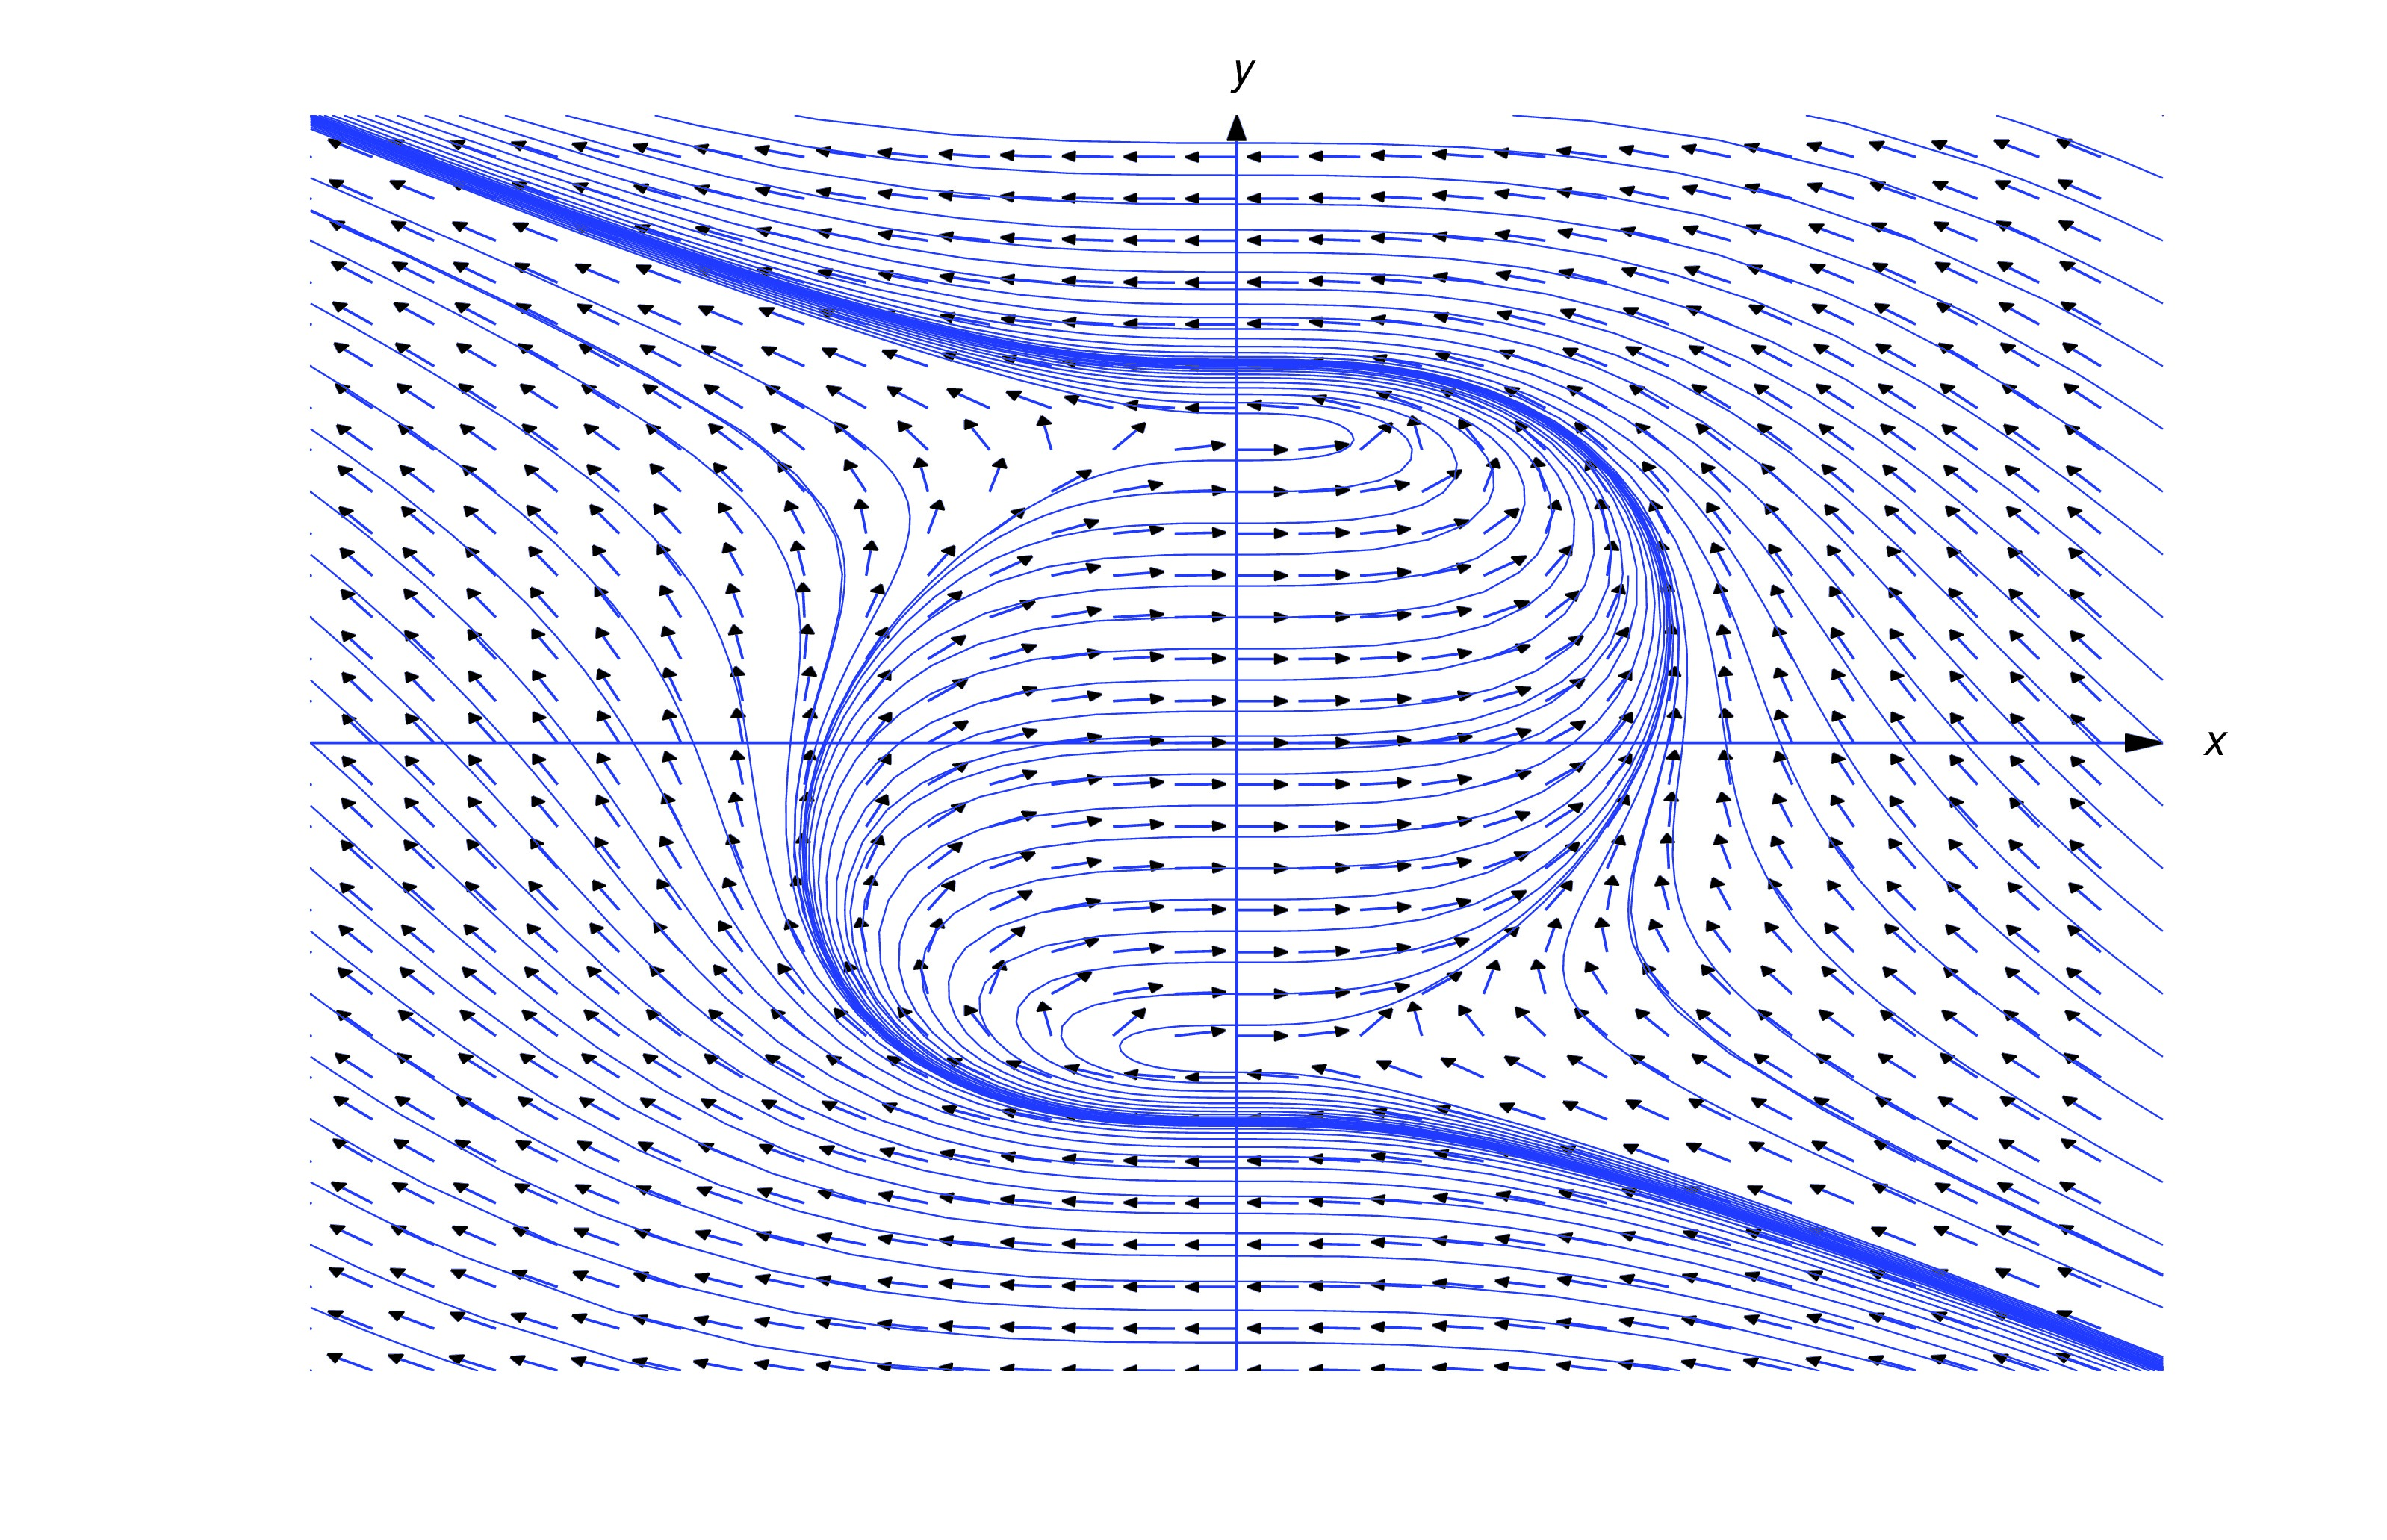
\includegraphics{fig010306.jpg}
\end{image}
The integral curves near the top and bottom are
solution curves. However, the integral curves near the middle are more
complicated. For example, the figure below shows the integral
curve through the origin. The vertices of the dashed rectangle are on
the circle $x^2+y^2=1$ ($a\approx.846$, $b\approx.533$), where all
integral curves of \eqref{eq:1.3.3} have infinite slope. 
\begin{image}
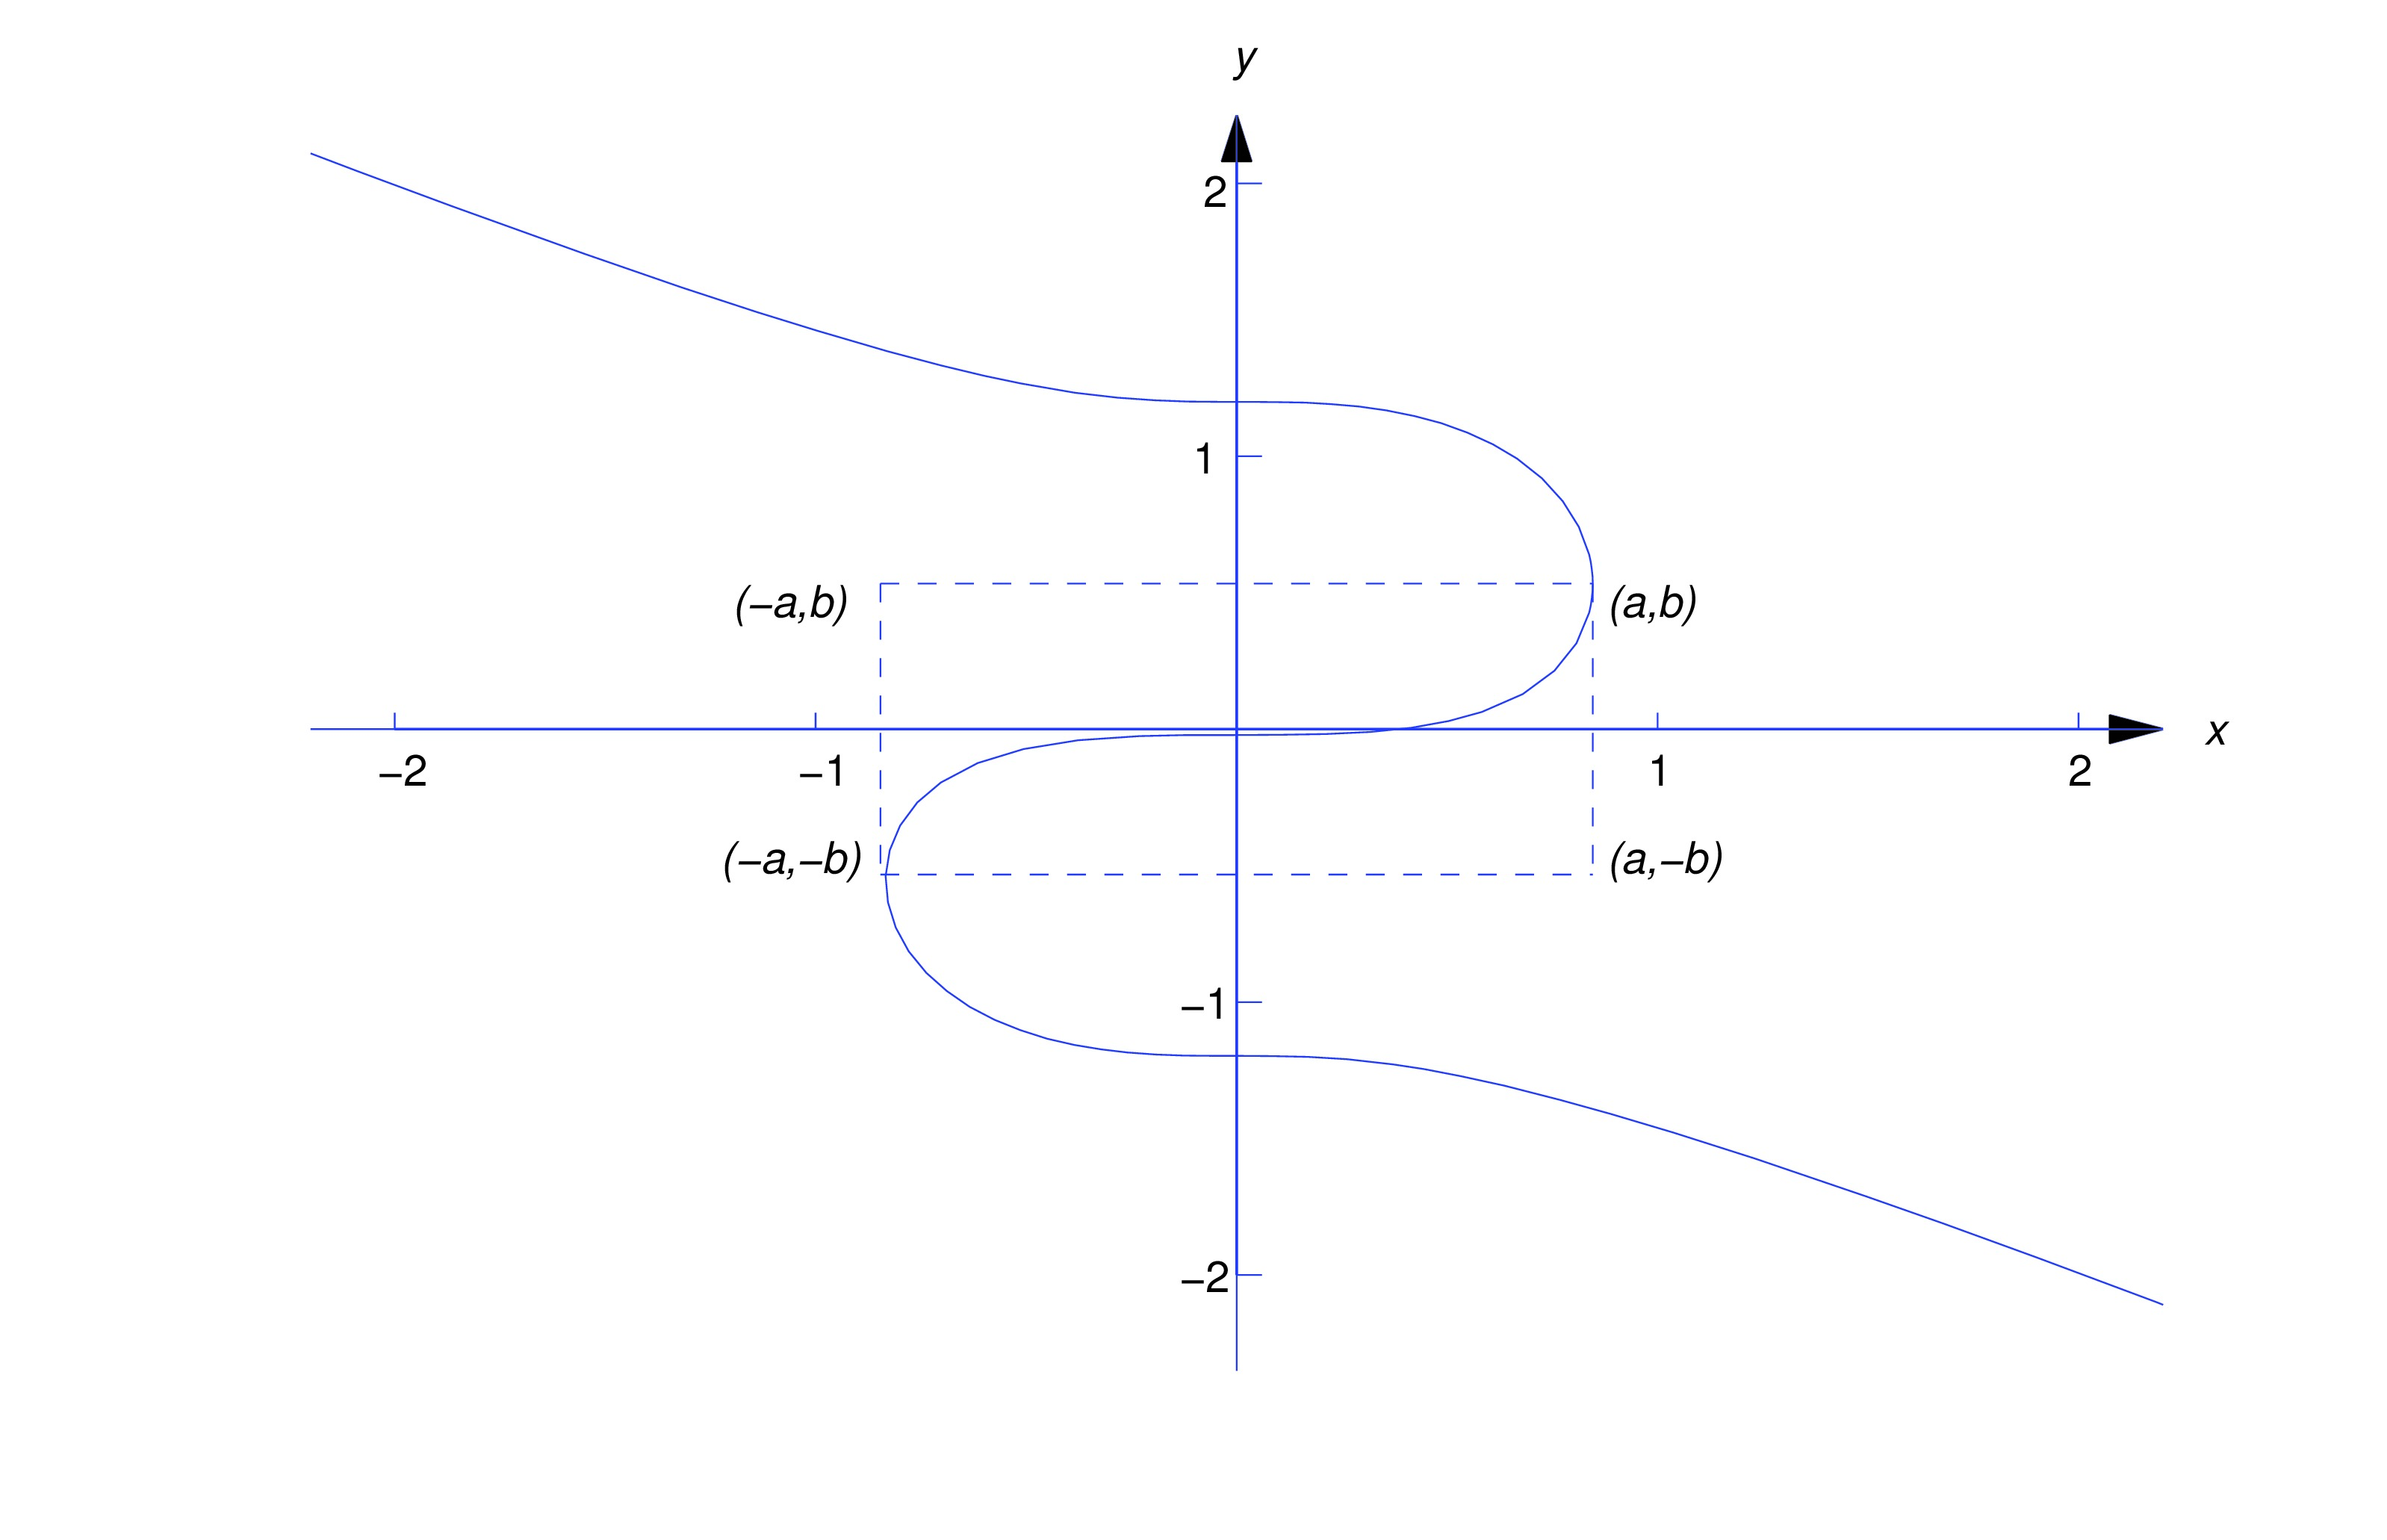
\includegraphics{fig010307.jpg}
\end{image}
There are
three solution curves of \eqref{eq:1.3.3} on the integral curve in the
figure: the segment above the level $y=b$ is the graph of a solution
on $(-\infty,a)$, the segment below the level $y=-b$ is the graph of a
solution on $(-a,\infty)$, and the segment between these two levels is
the graph of a solution on $(-a,a)$.

Even if $f$ is continuous and otherwise ``nice''
throughout $R$, your software  may require you to
reformulate the equation $y'=f(x,y)$ as
$$
\frac{dx}{dt}=1,\quad \frac{dy}{dt}=f(x,y),
$$
which is of the form \eqref{eq:1.3.5} with $A(x,y)=f(x,y)$ and
$B(x,y)=1$.

As you study from this book, you'll often be asked to use
computer software and graphics. 
%Exercises with this intent are marked
%as \Cex\, (computer or calculator required), \CGex\, (computer and/or
%graphics required), or \Lex\ (laboratory work requiring software
%and/or graphics).
 Often
you may not completely understand how the software does what it does.
This is similar to the situation most people are in when they drive
automobiles or watch television, and it doesn't decrease the value
of using modern technology as an aid to learning. Just be careful that
you use the technology as a supplement to thought rather than a
substitute for it.



\section*{Text Source}

\href{https://github.com/mooculus/calculus}{MOOCulus}, \href{https://github.com/mooculus/calculus/blob/6255bcdf3fae1b17972a7ae4883841bf25464c61/numericalMethods/digInSlopeFieldsAndEulersMethod.tex#L22}{Numerical Methods} (CC-BY-NC-SA)


Trench, William F., "Elementary Differential Equations" (2013). Faculty Authored and Edited Books & CDs. 8. (CC-BY-NC-SA)

\href{https://digitalcommons.trinity.edu/mono/8/}{https://digitalcommons.trinity.edu/mono/8/}


\end{document}